\documentclass[12pt]{article}

\usepackage[margin=1in]{geometry}
\usepackage[ampersand]{easylist}
\usepackage{tikz}
\usepackage{float}
\usepackage{fp}
\usepackage{listings}
\usepackage{amsmath,esint}
\usepackage{fancyhdr}
\usepackage[version=3]{mhchem}
\usepackage{textcomp}
\usepackage{mathtools}
\usepackage{multicol}
\usepackage[american]{circuitikz}
\usepackage{amsfonts}
\usepackage{mathtools}
\usepackage{multirow}
\usepackage{sectsty}
\usepackage{multicol}
\usepackage{lastpage}
\usepackage[font={small,it}]{caption}
\usepackage{array}
\usepackage{url}
\usepackage{amsmath}

\newcolumntype{L}[1]{>{\raggedright\let\newline\\\arraybackslash\hspace{0pt}}m{#1}}
\newcolumntype{C}[1]{>{\centering\let\newline\\\arraybackslash\hspace{0pt}}m{#1}}
\newcolumntype{R}[1]{>{\raggedleft\let\newline\\\arraybackslash\hspace{0pt}}m{#1}}
\pagestyle{fancy}
\lhead{ECE337 Project Phase 1 Report}

\cfoot{Page {\thepage} of \pageref{LastPage}}
\renewcommand{\headrulewidth}{0.4pt}
\renewcommand{\footrulewidth}{0.4pt}
\usetikzlibrary{decorations.markings,patterns}
\usetikzlibrary{arrows}

\setlength\parindent{0pt}
\setcounter{tocdepth}{2}
%\setcounter{section}{2}

\usepackage{titlesec}
\titleformat{\section}
{\normalfont\fontsize{14}{15}\selectfont\bfseries}{\thesection}{1em}{}[{\titlerule[0.5pt]}]
\titleformat{\subsection}
{\normalfont\fontsize{14}{15}\selectfont\bfseries}{\thesubsection}{1em}{}[{}]



\usepackage{tocloft}
\newcommand{\listequationsname}{List of Equations}
\newlistof{myequations}{equ}{\listequationsname}
\newcommand{\myequations}[1]{
    \addcontentsline{equ}{myequations}{\protect\numberline{\theequation}#1}\par}


\newcommand*{\plogo}{\fbox{$\mathcal{PL}$}} % Generic publisher logo

\newcommand*{\titleGP}{\begingroup % Create the command for including the title page in the document
\centering % Center all text
\vspace*{\baselineskip} % White space at the top of the page

\rule{\textwidth}{1.6pt}\vspace*{-\baselineskip}\vspace*{2pt} % Thick horizontal line
\rule{\textwidth}{0.4pt}\\[\baselineskip] % Thin horizontal line
{\bf \fontsize{17.5pt}{12pt}\selectfont {Handwritten Digit Recognizer using Neural Networks}}\\[0.5\baselineskip] % Title
{\large Phase 1 Project Proposal\\
    TA: Anirudh\\[4pt]
Wednesday | 11:30}

\rule{\textwidth}{0.4pt}\vspace*{-\baselineskip}\vspace{3.2pt} % Thin horizontal line
\rule{\textwidth}{1.6pt}\\[3\baselineskip] % Thick horizontal line



{\large\sc David Pimley} % Editor list
\\[0.5\baselineskip]
{\large\sc Chan Weng Yan} % Editor list
\\[0.5\baselineskip]
{\large\sc Dustin Andree} % Editor list
\\[0.5\baselineskip]
{\large\sc Vadim Nikiforov} % Editor list
\\[3\baselineskip]
{\large\sc ECE 33700} % Editor list
\\[0.5\baselineskip]
{\large\sc 2/12/2018} % Editor list
\\\vspace{15\baselineskip}
{\itshape Purdue University\\ Computer Engineering\par} % Editor affiliation

\vfill % Whitespace between editor names and publisher logo

{\large }\par % Publisher

\endgroup}



    \begin{document}
\pagestyle{plain}
	\titleGP
    \newpage
    \pagestyle{fancy}

    \section{Executive Summary}
    This project idea is a digit recognizer. It is designed to work with images consistent with the MNIST dataset, so it accepts 14$\times$14 px grayscale images, and outputs a detected digit. It accepts an image, and a list of weights and biases for the network connections. While it doesn't have an internal method for training, it outputs a cost function for each set of images, allowing for it to be connected to an external training module. Furthermore, using SPI, the network model can be reprogrammed on the fly. Digit recognition is a very useful application, as it allows for devices to interpret data ranging from checks to signs to handwritten notes. Machine learning allows for very high accuracy for digit detection, and when applied to digit recognition can handle a wide range of fonts and handwriting styles. However, due to the structure of neural networks, sequential computation such as what is found in microcontrollers is not effective for a neural network. Instead, devices such as GPUs are often used due to their capacity for parallel computation. This device uses an architecture specialized just for multiplying weights and adding inputs, allowing for much faster computation for digit recognition. While on a microcontroller this system would require tens of thousands of sequential multiplications, on an ASIC it will be possible to run calculations in parallel, and implement pipelining for addition and multiplication. This is done by taking advantage of the MapReduce procedure, where in this case the mapping is applying weights to the biases, and the reduction is adding together all the inputs to a sigmoid, and then calculating the sigmoid output (which can be done by a lookup table.) Finally, this device allows for training to be done on separate hardware, which typically requires far more computational power than detection, and then allows the trained model to be uploaded on the fly using a standard interface (In this case, SPI) allowing for flexible operation.\\

    To complete this design of a digit recognizer, the following will be needed:


    \begin{itemize}
        \item SST39LF200A ($\times$16) Multi Purpose Flash Datasheet
        \item Reference Standard Cell Simulation Library for Mapped Design Verification
        \item Reference Standard Cell Technology Library for Final Design Layout Verification
        \item Verilog HDL Simulation and Design Synthesis Tool Chain
    \end{itemize}




The following design proposal will include:

\begin{itemize}
    \item A top level system usage diagram for an example configuration/usage of the digit recognizer circuit.
    \item The standards/algorithms to be implemented by the digit recognizer circuit.
    \item The design pinout of the neural network, and input output signals with their associated access codes.
    \item The specific design architecture to be utilized by the digit recognition circuit.
\end{itemize}

\section{Design Specifications}
\subsection{System Usage}
\subsubsection{System Usage Diagram\label{sec:sysuse}}
\begin{figure}[H]
    \centering
    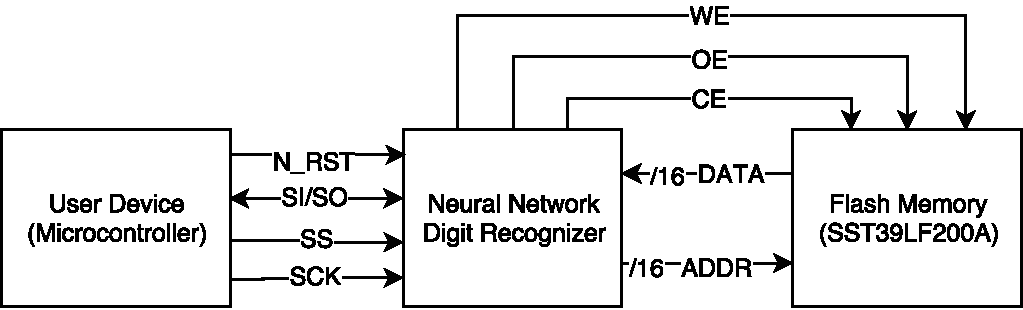
\includegraphics[width=0.7\textwidth]{top_level_block.pdf}
    \caption{Example system usage diagram of neural network digit recognizer}
    \label{fig:top}
\end{figure}

This design is intended to accelerate the recognition of digits by implementing a neural network in an ASIC, allowing for parallel computation. However, the functionality can only be useful when interfaced with a general purpose computing device. The application depicted in the system usage diagram shows the recognizer interfacing with a microcontroller via SPI. An additional necessary module is flash memory. This is used to store the weights and biases for the neural network, and is used to prevent the need to reupload the model every time. If the model needs to be changed, then it can be uploaded directly to the flash memory using an external chip. The microcontroller in this example would be used as a control device. While the majority of the work being done is accomplished within the Neural Network Block, the control functionality comes from the user device performing the following tasks:



\begin{enumerate}
    \item If necessary, reset the registers (everything but the Flash Memory)
    \item Using the SS, the SPI register will choose which operation to be done. The four operations are:
        \begin{enumerate}
            \item Let the digit recognizer know that image data will be sent over MOSI.
            \item Ask the digit recognizer for the result of the previous operation.
            \item Ask the digit recognizer for the cost of the previous operation.
            \item Let the digit recognizer know that the weights and bias will be changed in which case the registers will need to be flushed.
            \item Let the digit recognizer know the expected label\footnote{Label is defined as the expected output digit value for a given image.} of each image (needed for calculating the cost\footnote{Cost is defined as the mean squared error between the expected and calculated labels for a set of digit images.} output)
        \end{enumerate}
\end{enumerate}
\newpage

\subsubsection{Implemented Standards and Algorithms\label{sec:standards}}

\subsubsection*{SPI:}

\begin{easylist}[itemize]
& Synchronous serial communication between the user device and the neural network digit recognizer.
& MOSI/MISO compatible with external device (such as a microcontroller).
\end{easylist}



\subsubsection*{Flash Memory:}

\begin{easylist}
& Permanent storage memory for bias/weight data.
& Communicates with a 16 bit address bus, a 16 bit data bus, and read,write, and chip enable lines.
\end{easylist}



\subsubsection*{Pipelining:}

\begin{easylist}
& ``Pre-Processing'', once values from a register are used, those values are updated with the next value to be utilized, if a calculation requires multiple cycles.
& Allows the same arithmetic unit to be used for multiple calculations at once.
\end{easylist}



\subsubsection*{ALU:}

\begin{easylist}
& Fixed Point Addition
&& 16 bit signed addition used for bias addition to each weighted pixel.
& Fixed Point Multiplication
&& Extension of Fixed Point Addition, used to multiply matrices in parallel within the digit recognizer to speed up processing.
& Sigmoid Function
&& Used for the output of the sigmoid neuron registers, calculated using a lookup table.
\end{easylist}

\subsubsection*{Signals:}


\begin{table}[H]
    \centering
\begin{tabular}[]{|c|l|}
    \hline
Command Code & Description \\ \hline \hline
\texttt{1'b000} & New image data is being input over MOSI \\ 
\texttt{1'b001} & New expected label is being input over MOSI \\ 
\texttt{1'b010} & Output the cost of the last operation \\ 
\texttt{1'b011} & Output the result of the last operation \\
\texttt{1'b100} & The weights/biases have changed, flush registers \\ \hline
\end{tabular}
    \caption{Device instruction bits for SPI}
    \label{tab:instruction}
\end{table}

\subsection{Pinout}
\begin{table}[H]
    \centering
    \begin{tabular}[]{|l|l|l|p{250pt}|}
        \hline
        Signal Name & Direction & \# Bits & Description \\ \hline \hline
        \texttt{PWR} & power & N/A & System Power\\
        \texttt{GND} & ground & N/A & System \\
        \texttt{CLK} & in &1 & System Clock\\
        \texttt{N\_RST} & in & 1 & Active low reset signal\\\hline
    \end{tabular}
    \caption{Miscillaneous Pinouts}
    \label{tab:misc}
\end{table}

\begin{table}[H]
    \centering
    \begin{tabular}[]{|l|l|l|p{250pt}|}
        \hline
        Signal Name & Direction & \# Bits & Description \\ \hline \hline
        \texttt{MISO} & out & 1 & Master in slave out signal\\
        \texttt{MOSI} & in  & 1 & Master out slave in signal\\
        \texttt{SCK} & in & 1 & SPI clock\\
        \texttt{SS} & out& 1 & Slave select Signal\\\hline
    \end{tabular}
    \caption{User device pinouts}
    \label{tab:user}
\end{table}

\begin{table}[H]
    \centering
    \begin{tabular}[]{|l|l|l|p{250pt}|}
        \hline
        Signal Name & Direction & \# Bits & Description \\ \hline \hline
        \texttt{WE} & out & 1 & Write Enable Signal\\
        \texttt{OE} & out & 1 & Output Enable Signal\\
        \texttt{CE} & out& 1 & Chip Enable Signal\\
        \texttt{DATA} & in & 16 & Bias/weight data from the external flash memory\\
        \texttt{ADDR} & out & 16 & Address for flash memory\\\hline
    \end{tabular}
    \caption{Flash memory pinouts}
    \label{tab:flash}
\end{table}

The signals specified in Table~\ref{tab:misc} represent any signals necessary for the chip to be powered and clocked. These are not labeled in the design architecture. Next, the pins in Table~\ref{tab:user} are the signals that are exposed to any device that will use the neural network for detecting digits. Finally, the pins in Table~\ref{tab:flash} are the signals that are necessary for the neural network to interface with its flash memory.

\newpage
\section{Design Architecture}
\begin{figure}[H]
    \centering
    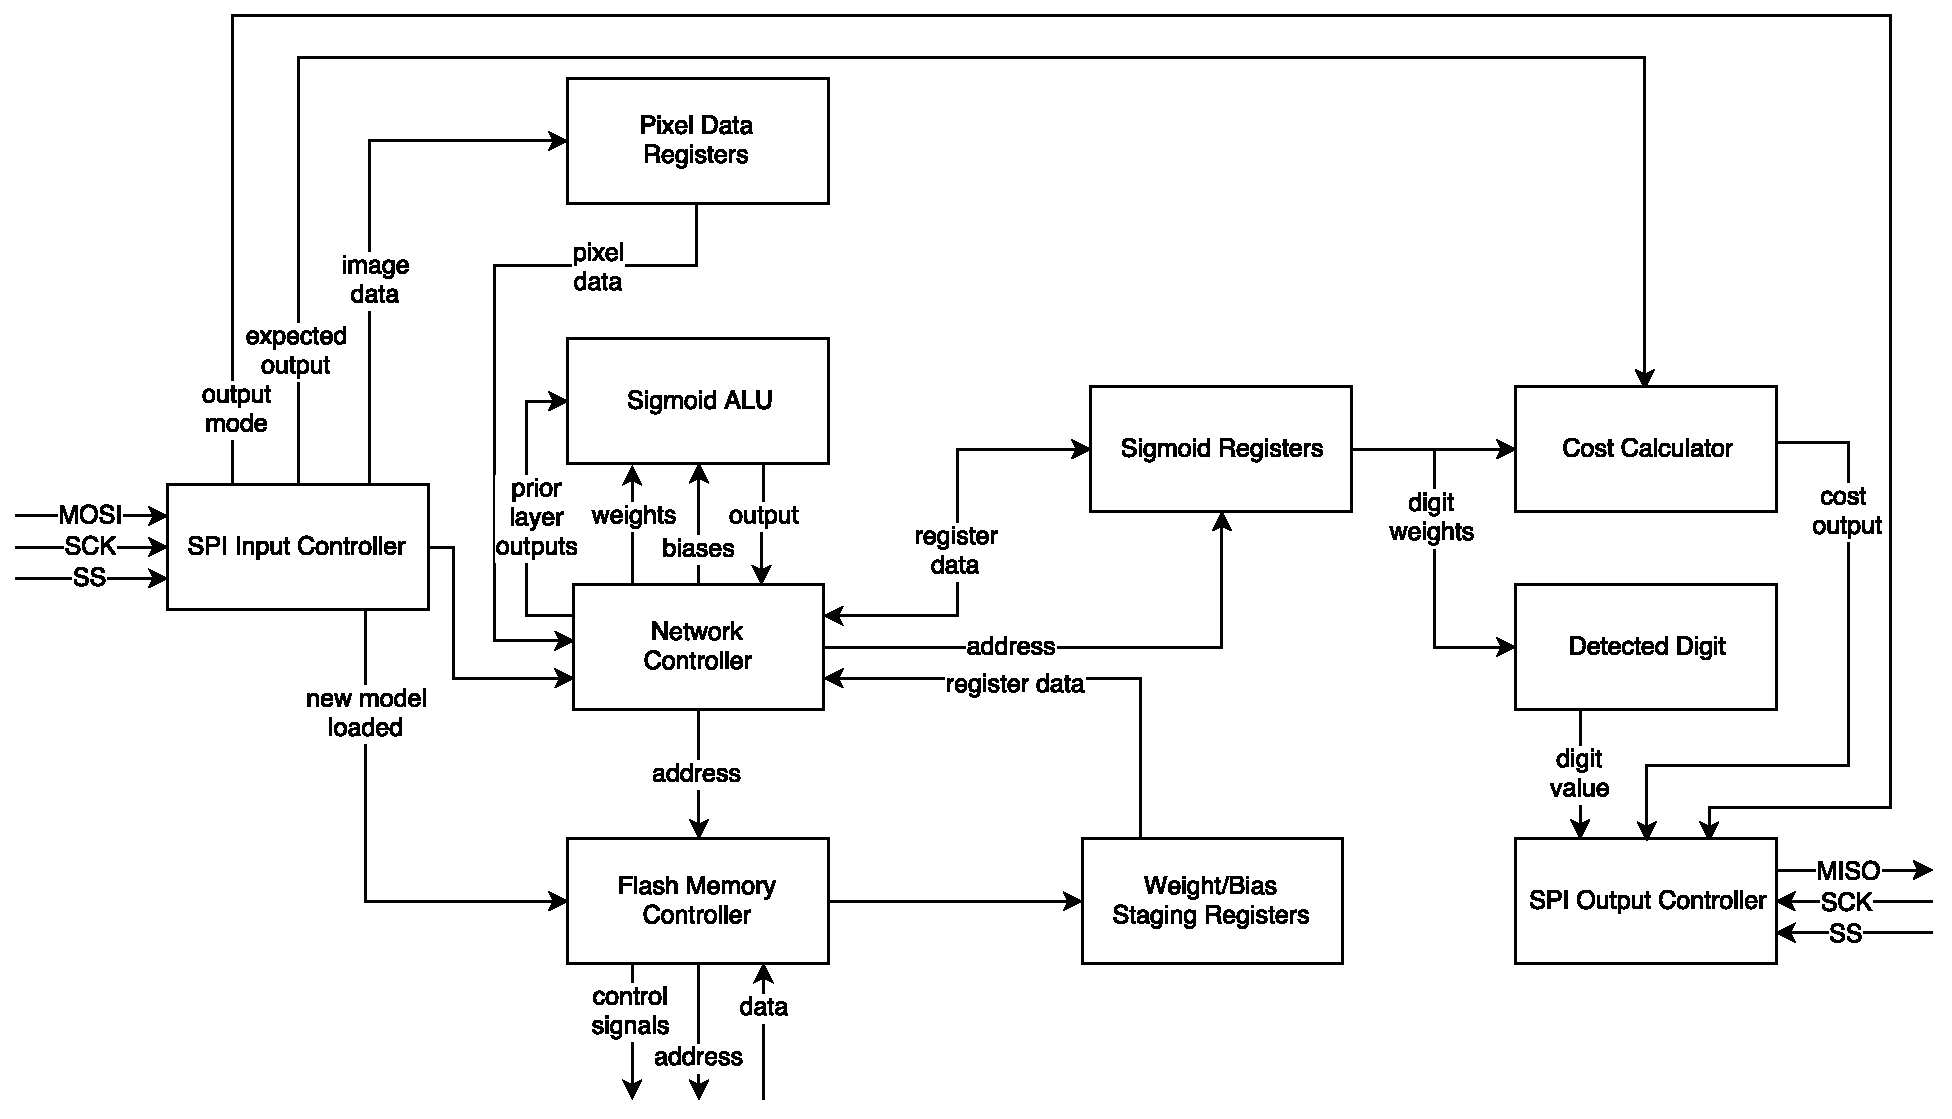
\includegraphics[width=\textwidth]{digit_recognizer_2.pdf}
    \caption{Digit recognition circuit design architecture}
    \label{fig:detail}
\end{figure}
The design architecture of the digit recognition circuit is shown in Figure~\ref{fig:detail}. All input first is fed to the SPI Input Controller where the data is filtered into one of a few different blocks. Each data destination block is determined by the input code. The input codes are laid out in Section~\ref{sec:standards}. For the standard operating mode (output), image data is fed into the input controller and sent to a staging register used specifically for holding the data of each image. The network controller uses this data as well as data from the weight/bias staging registers (loaded from flash memory) to be input into the Sigmoid ALU to calculate probabilities for each number, \textit{i.e.}~0-9. Depending on if the microcontroller asks for the cost analysis of the previous operation, the cost can also be output on the MISO line used for outputting the detected digit.









    \end{document}
